% Load the kaobook class
\documentclass[
	fontsize=10pt, % Base font size
	twoside=false, % Use different layouts for even and odd pages (in particular, if twoside=true, the margin column will be always on the outside)
	%open=any, % If twoside=true, uncomment this to force new chapters to start on any page, not only on right (odd) pages
	secnumdepth=1, % How deep to number headings. Defaults to 1 (sections)
]{kaobook}

% Choose the language
\usepackage[english]{babel} % Load characters and hyphenation
\usepackage[english=british]{csquotes}	% English quotes

% Load packages for testing
\usepackage{blindtext}
%\usepackage{showframe} % Uncomment to show boxes around the text area, margin, header and footer
%\usepackage{showlabels} % Uncomment to output the content of \label commands to the document where they are used

% Load the bibliography package
\usepackage{kaobiblio}
\addbibresource{library.bib} % Bibliography file

% Load mathematical packages for theorems and related environments
\usepackage{kaotheorems}

% Load the package for hyperreferences
\usepackage{kaorefs}

% To be able to include Tikz files
% \usepackage{standalone}

% To typeset date and time
\usepackage{datetime2}
\DTMsetstyle{ddmmyyyy}

% For logos on titlepage.
\usepackage{tabularx}

% \newcommand{\ie}{i.\,e.\,}
% \newcommand{\Ie}{I.\,e.\,}
% \newcommand{\eg}{e.\,g.\,}
% \newcommand{\Eg}{E.\,g.\,}

% For logos on title page
\newcolumntype{u}{>{\hsize=0.56\hsize}X}
\newcolumntype{v}{>{\hsize=0.44\hsize}X}

% For check/x-marks
\usepackage{pifont}% http://ctan.org/pkg/pifont
\newcommand{\cmark}{\ding{51}}%
\newcommand{\xmark}{\ding{55}}%

\graphicspath{{images/}{./}} % Paths where images are looked for

\makeindex[columns=3, title=Alphabetical Index, intoc] % Make LaTeX produce the files required to compile the index


\begin{document}

%----------------------------------------------------------------------------------------
%	BOOK INFORMATION
%----------------------------------------------------------------------------------------

\titlehead{Draft}
\title[Deep learning on higher harmonic generation images for regression and pathology]{Deep learning on higher harmonic generation images for regression and pathology} % {\normalfont\texttt{kaobook}}
\author[SJ]{Siem de Jong}
\date{\today}
\publishers{}

%----------------------------------------------------------------------------------------

\frontmatter % Denotes the start of the pre-document content, uses roman numerals

%----------------------------------------------------------------------------------------
%	COPYRIGHT PAGE
%----------------------------------------------------------------------------------------

\makeatletter
\uppertitleback{\@titlehead} % Header

\lowertitleback{
	\textbf{Disclaimer} \\
	You can edit this page to suit your needs. For instance, here we have a no copyright statement, a colophon and some other information. This page is based on the corresponding page of Ken Arroyo Ohori's thesis, with minimal changes.

	\medskip

	\textbf{No copyright} \\
	\cczero\ This book is released into the public domain using the CC0 code. To the extent possible under law, I waive all copyright and related or neighbouring rights to this work.

	To view a copy of the CC0 code, visit: \\\url{http://creativecommons.org/publicdomain/zero/1.0/}

	\medskip

	\textbf{Colophon} \\
	This document was typeset with the help of \href{https://sourceforge.net/projects/koma-script/}{\KOMAScript} and \href{https://www.latex-project.org/}{\LaTeX} using the \href{https://github.com/fmarotta/kaobook/}{kaobook} class.

	\medskip

	\textbf{Publisher} \\
	First printed in May 2019 by \@publishers
}
\makeatother

%----------------------------------------------------------------------------------------
%	DEDICATION
%----------------------------------------------------------------------------------------

\dedication{
	The harmony of the world is made manifest in Form and Number, and the heart and soul and all the poetry of Natural Philosophy are embodied in the concept of mathematical beauty.\\
	\flushright -- D'Arcy Wentworth Thompson
}

%----------------------------------------------------------------------------------------
%	OUTPUT TITLE PAGE AND PREVIOUS
%----------------------------------------------------------------------------------------

% Note that \maketitle outputs the pages before here
% \maketitle
%*******************************************************
% Titlepage
%*******************************************************
\begin{titlepage}
    \pdfbookmark[1]{Titlepage}{titlepage}
    % if you want the titlepage to be centered, uncomment and fine-tune the line below (KOMA classes environment)
    % \begin{addmargin}[-1.8cm]{-4.4cm}
    \begin{center}

        \vfill

        % \begin{addmargin}[-2cm]{-2cm}
        \begingroup
        \centering
        % \color{CTtitle}\spacedallcaps{\myTitle}
        \usekomafont{title}{\huge Deep learning on higher harmonic generation images for regression and pathology \par}
        \endgroup
        % \end{addmargin}

        % \spacedlowsmallcaps{\mySubtitle} \bigskip

        % \spacedlowsmallcaps{\myName \\ UvA: \myStudentNumberOne \\ VU: \myStudentNumberTwo} \bigskip
        \usekomafont{author}{Siem de Jong \par} \bigskip

        Faculty of Science, University of Amsterdam \\
        Faculty of Science, Vrije Universiteit Amsterdam \\ \smallskip
        LaserLaB Amsterdam, \emph{Biophotonics and Biomedical Imaging}

        \vfill

        % Name and logo of institute
        
\includegraphics[width=6cm]{frontbackmatter/images/laserlab-logo.pdf}

        \vfill

        Report Master Project Physics and Astronomy \\
        \emph{track Biophysics and Biophotonics} \\
        60 EC \\
        % Conducted between 05--09--2022 and xx--xx--2023
        Conducted between \DTMdisplaydate{2022}{09}{05}{-1} and DD-MM-YYYY%\DTMdisplaydate{2023}{07}{01}{-1}

        \vfill

        \begin{tabular}{rl}
            Daily supervisor & Dr.\ rer.\ nat.\ P.\ J.\ González     \\
            Examiner         & Prof.\ dr.\ M.\ L.\ Groot             \\
            Second reviewer  & Dr.\ rer.\ nat.\ D.\ W.\ A.\ Hillmann
        \end{tabular}

        \vfill

        % Change this date upon submission to fix the date.
        \today

        \vfill

        \begin{tabularx}{\textwidth}{vu}
            % \raisebox{-.5\dimexpr\totalheight-\ht\strutbox}{...} % bring down images so they align. [https://tex.stackexchange.com/questions/314821/vertically-and-horizontally-align-image-inside-table]
            \raisebox{-.5\dimexpr\totalheight-\ht\strutbox}{
\includegraphics[width=\hsize]{frontbackmatter/images/vu-logo.pdf}} &
            \raisebox{-.5\dimexpr\totalheight-\ht\strutbox}{
\includegraphics[width=\hsize]{frontbackmatter/images/uva-logo.pdf}}
        \end{tabularx}

    \end{center}
    % \end{addmargin}
\end{titlepage}

%----------------------------------------------------------------------------------------
%	PREFACE
%----------------------------------------------------------------------------------------

\chapter*{Preface}

\blindtext

%----------------------------------------------------------------------------------------
%	TABLE OF CONTENTS & LIST OF FIGURES/TABLES
%----------------------------------------------------------------------------------------

\begingroup % Local scope for the following commands

% Define the style for the TOC, LOF, and LOT
%\setstretch{1} % Uncomment to modify line spacing in the ToC
%\hypersetup{linkcolor=blue} % Uncomment to set the colour of links in the ToC
\setlength{\textheight}{230\vscale} % Manually adjust the height of the ToC pages

% Turn on compatibility mode for the etoc package
\etocstandarddisplaystyle % "toc display" as if etoc was not loaded
\etocstandardlines % "toc lines as if etoc was not loaded

\tableofcontents % Output the table of contents

\listoffigures % Output the list of figures

% Comment both of the following lines to have the LOF and the LOT on different pages
\let\cleardoublepage\bigskip
\let\clearpage\bigskip

\listoftables % Output the list of tables

\endgroup

%----------------------------------------------------------------------------------------
%	MAIN BODY
%----------------------------------------------------------------------------------------

\mainmatter % Denotes the start of the main document content, resets page numbering and uses arabic numbers
\setchapterstyle{kao} % Choose the default chapter heading style

\pagelayout{wide} % No margins
% \addpart[Skinstression]{Strain-stress regression on \\ second harmonic generation images \\ using {\normalfont\texttt{Skinstression}}}
\addpart[Skinstression]{Development and validation of a strain-stress regression model on second harmonic generation images from old adult skin tissue}
\pagelayout{margin} % Restore margins

\chapter{Introduction}

Human skin tissue is mostly built by collagen and elastin.
Second harmonic generation (SHG) imaging allows to image collagen and two-photon excitation microscopy (2PEF).
Setups have been built to collect SHG and 2PEF signals simultaneously, allowing for rich skin tissue imaging.
Collagen fibers are clearly visible.
Previous studies have shown that collagen and not elastin dictates the stretching ability of skin tissue.
A recent study (Mengyao) aims to show the connection between collagen density and amount of stretching.
To measure the stretch of skin tissue, mechanical measurements have to be performed.
SHG images of the collagen networks in conjuction with the strain-stress curves suggest that the images already contain stretch information.
Retrieving complex features from labelled images can be done using supervised deep learning.
Supervised deep learning is considered a black-box technique that aims to learn a mapping from input to output.
With the SHG images and corresponding stress-strain measurements at hand, \texttt{Skinstression} is developed with the ultimate goal to replace mechanical measurements on skin tissue to quantify skin stretch.
Efforts to develop such a model have already been made by A.\ Soylu.
However, those methods do not consider complete separation of training and test sets in both inference and label creation, possibly leading to biased results.
Moreover, only one slice of larger image stacks have been used.
Using more, if not all, images of a stack might lead to a more robust model.
This study extends Soylu's model.

\chapter{Theory}

\section{Dropout}\label{sec:dropout}


\section{Batch normalization}\label{sec:bn}
Batch normalization (BN)~\cite{Ioffe2015} is a technique to shift and scale batches akin to standardization.
It can be implemented as a layer in any neural network.
Per minibatch and per dimension, the mean and standard deviation of the input are calculated.
Then, the input is standardized with
\begin{equation}
    \hat{x}_i = \frac{x_i - \mu_\mathcal{B}}{\sqrt{\sigma_\mathcal{B}^2 + \epsilon}},
\end{equation}
where $\mu_\mathcal{B}$ and $\sigma_\mathcal{B}$ are the mean and unbiased standard deviation of the batch, and $\epsilon$ is a small number for numerical stability when the variance is small.
The standardized input is then mapped through
\begin{equation}
    y_i = \gamma \hat{x}_i + \beta,
\end{equation}
where $\gamma$ and $\beta$ are learnable parameters learned in a sub-network.

\section{Activation functions}\label{sec:activations}

\begin{enumerate}
    \item heaviside
    \item logistic curves
    \item vanishing gradient problem -> relu
\end{enumerate}

\subsection{Rectified linear unit}\label{subsec:relu}
To overcome the vanishing gradient problem, non-saturating activation functions can be used.
One such function is the rectified linear unit (ReLU).
It is defined as
\begin{equation}
    f(x) = x^+ = \max(0, x),
\end{equation}
such that only the positive arguments keep their value.

\section{Pooling}\label{sec:pooling}
Pooling is a form of nonlinear downsampling.
Typically, a convolution kernel is moved over the input with a stride as big as the kernel itself.
This ensures that the downsampling considers measures of input sub-regions.

\subsection{Maxpool}\label{subsec:maxpool}
The most common form of pooling is maxpooling (ref).
The kernel finds the maximum value in sub-regions and maps these maximum values per sub-region to a new image.\marginpar{TODO: function}
For example, a $\SI{2}{px}\times\SI{2}{px}$ maxpool kernel on a $\SI{10}{px}\times\SI{10}{px}$ image outputs a $\SI{5}{px}\times\SI{5}{px}$ image.


% --------------------------------------------------
% Loss functions
% --------------------------------------------------

\section{Loss functions}
Backpropagation needs a loss to learn in which direction to update weights.
There is a variety of loss functions available (ref review).

\subsection{Mean absolute error}
One of the most straightforward techniques of calculating the loss is the mean absolute error (MAE).
It measures the average difference between every prediction and target, like
\begin{equation}
    \mathrm{MAE} = \frac{1}{n} \sum_{i=1}^{n} |y_i - y'_i|,
\end{equation}
where $n$ is the number of targets per sample, $y$ the prediction and $y'$ the target.

The MAE loss is forgiving, i.\ e.\ outliers are weighted as much as predictions close to the target.
In training a neural network, focusing on outliers is assumed to be beneficial, as those are the cases that the model has difficulty with (ref).

\subsection{Mean square error}
To overcome the forgiving nature of the MAE loss, the mean square error (MSE) can be used.
It measures the average squared difference between every prediction and target, like
\begin{equation}
    \mathrm{MSE} = \frac{1}{n} \sum_{i=1}^n (y_i - y'_i)^2.
\end{equation}

\subsection{Focal MSE}
To give even more focus on the hard targets, giving them more importance than easy targets can be done through the focal MSE loss (FL)~\cite{Lu2022}.
To give less importance to the easier targets, FL follows
\begin{equation}
    FL = \left(\frac{2}{1 + e^{-\beta |y - y'|}} - 1 \right)^\gamma (y_i - y'_i)^2,
\end{equation}
where increasing $\gamma$ increases the number of targets regarded as easy and $\beta$ regulates the speed with which the first part of the curve increases (make fig).

% --------------------------------------------------
% Label density smoothing
% --------------------------------------------------

\section{Label density smoothing}
The targets calculated with logistic curve fitting result in a non-uniform distribution.
Data imbalance reduces the ability of a neural network to learn outliers.
This may have significant impact on the test results.
To deal with imbalanced data, various techniques have been developed.
One of those techniques is label density smoothing (LDS)~\cite{yang2021delving}.
It is specifically designed for deep neural networks to learn from imbalanced continuous targets.

\newcommand{\edtl}{$\tilde{p}(y')$ }
LDS computes the effective label density distribution,
\begin{equation}
    \tilde{p}(y') = \int_Y k(y, y')p(y)dy,
\end{equation}
where $k(y,y')$ is a symmetric kernel, $p(y)$ the number of label $y$ present in the training data and \edtl the effective density of target label $y'$.
Reweighting the loss function with the inverse (square root) of \edtl addresses target imbalance.

\subsection*{layout}
\begin{enumerate}
    \item deep neural network as regressor
    \item image quality
          \begin{enumerate}
              \item entropy
              \item ...
          \end{enumerate}
    \item noise2void
    \item road to logistic curve
    \item label density smoothing
    \item loss functions
\end{enumerate}
\chapter{Methods}
\begin{enumerate}
    \item TODO: SQUASH SECTION BELOW INTO FEWER SECTIONS AND MAKE IT FLOW
    \item TODO: DETAIL
\end{enumerate}

\section{Sources of data}

Data is obtained in previous studies by A.\ Soylu, M.\ Zhou, and Ludo X\marginnote{What is Ludo's name? And ref to paper?} at the Medical Imaging center of the VUmc, Amsterdam.
\marginnote{Agreement?}
Human thigh and abdomen skin tissue were excised.
Pieces of these tissues were imaged with multiphoton microscopy and their stress-strain response curves were measured mechanically.
Data is acquired in batches from April 2021 until July 2022.
Development and testing data come from the same source.

Cadavers were eligible for thigh skin excision and abdomen skin is cut during plastic surgery.\marginnote{is this true?}
It is unknown if individuals received treatment relevant for this study.


\section{Data preparation}\label{sec:skin_data_prep}

\subsection{Preprocessing}

Depth stack images with a size of $\qty{1000}{px}\times\qty{1000}{px}$of all skin tissues were kindly provided by M.\ Zhou.
All stacks were separated into slices.

Images consist of three channels: third and second harmonic generation, and autofluorescence.
The SHG channel is chosen as it is assumed to only contain collagen information.

The SHG images are enhanced with contrast limited adaptive histogram equalization (CLAHE) \cite{Zuiderveld1994ContrastLA} using scikit-image \cite{scikit-image} to equalize importance of dark and bright regions.

The enhanced images are then transformed with a Yeo-Johnson transform such that the histogram of all images is as normal as possible.

The transformed images are standardized by subtracting the total mean and total standard deviation of the complete transformed image set, like
\begin{equation}
    X_\mathrm{out} = \frac{X_\mathrm{in} - \mu}{\sigma},
\end{equation}
where
\begin{equation}
    \mu = \frac{1}{N} \sum_i \sum_j \sum_k X_{i,j,k},
\end{equation}
and
\begin{equation}
    % \sigma = \sqrt{\frac{1}{N} \sum_{i,j,k} X_{i,j,k}^2 - \left(\frac{1}{N} \sum_{i,j,k} X_{i,j,k}\right)^2},
    \sigma = \sqrt{\frac{1}{N} \sum_i \sum_j \sum_k \left(X_{i,j,k} - \mu\right)^2},
\end{equation}
with $N$ the total number of pixels, $k$ an individual image and $i,j$ the pixel in the horizontal and vertical dimension, respectively.

The images are downsampled to $\qty{258}{px}\times \qty{258}{px}$ to fit into the neural network.

\subsubsection{Image selection}
SHG microscopy images from skin tissue suffer from optical phenomena.
The most evident problem is that imaging deeper into the tissue, photons are detected with less spatial accuracy thanks to scattering.
The deeper photons travel into tissue, the more possible paths photons can take to return to the detector.
Moreover, the chance of photons getting absorbed by the tissue increases with penetration depth.
Therefore, less photons get reflected from deeper tissue.

To counter these optical effects, inspired by \textcite{Koho2016} and \textcite{Blokker2022}, measures to quantify image quality can be obtained.
With this, images can be sorted to this measure and the top $k$ images with best quality can be used to train the network, thus excluding noise.

Candidates for this measure are Shannon entropy, kurtosis, and skew for reasons explained in \ref{subsec:imq}
These quality measures are calculated per image, such that the quality measure can be validated by observing manually.

\subsubsection{Image denoising}
Another optical disadvantage of multiphoton microscopy is the occurrence of noise.\marginnote{Look up sources of noise.}

Unfortunately, obtaining clearer images is hard.
Given the experimental setup as in (ref\marginnote{Actually refer to the paper describing the setup, which is written by whom?!}), one way to reduce noise in the image is to use more photons.
Either by averaging more images or increasing the amount of photons per image.
Increasing the amount of photons penetrating the tissue increase the risk of damaging the tissue.

Another way to deal with noisy images is to process the images.
Promising denoising neural networks have been developed.
The difficulty with this is that clean target data for supervised training is often not available in a biomedical setting.
To counteract this, Noise2Noise (N2N) \cite{Lehtinen2018} was developed.
Noise2Void N2V \cite{Krull2019}, a successor of N2N, does not rely on pairs of noisy images.
Instead it only needs one image and corrupts it to use as target and learns a mapping between the noisy image and the newly created noisy image.
This is useful if only one biomedical image is available.\marginnote{If denoised is used, move parts of this section to a theory section and refer to it here.}

The original N2V model produces a checkerboard pattern.
Noise2Void2 (N2V2) \cite{Hock2022} is an extension to N2V and reduces this artifact.\marginnote{Actually didn't do denoising, but if done, describe how here :)}

\subsection{Data augmentation}

To make the model more robust, data augmentation is applied.
Before the downsampling, the preprocessed images are cropped randomly from $\qty{1000}{px}\times \qty{1000}{px}$ to $\qty{700}{px}\times \qty{700}{px}$ preserving the aspect ratio.
The global brightness is adjusted randomly with $\pm \qty{30}{\percent}$.
The images are then randomly mirrored horizontally and vertically with a probability of \qty{50}{\percent}.

\section{Outcome}
The strain-stress response curves of individual skin tissue pieces were the outcome of interest.
The prediction is assessed by comparing it with measured strain-stress curves.\marginnote{Describe this comparison}
The measurement is done mechanically by an experimentalist.
The mechanical measurement itself is blind to clinical information.

\section{Predictors}\label{sec:skin_predictors}

% --------------------------------------------------
% SEARCHING FOR A SIMPLE SKIN STRAIN-STRESS MODEL
% --------------------------------------------------

\subsection{Searching for a simple skin strain-stress model}

Supervised learning requires targets for the model to train on.
Ideally, individual targets allow for physical interpretation and can together describe all the available data.

\subsubsection{Empirical strain-stress regions}
Although skin tissue has a complex nature, measurements to quantify skin stretch show similar features.
Measurements always show three domains: the toe, heel and leg domain (see fig.).
The toe region is at the very start of the curve.
This region is seems relatively flat as the fiber network consists of mostly unstretched fibers.
Therefore, the fibers cannot exert force as a reaction to external stretching force.
However, in the heel region where skin tissue is stretched more, fibers can exert more force.
When enough force is exerted on the tissue, fibers stretch maximally and fibers react with maximum force in the leg region.
This region is observed to be roughly linear.
Overstretching the tissue then breaks the fiber network, decreasing the possibility to exert force.

\subsubsection{Exponential}
Strain-stress curves can be also be visualized by showing the log derivative of stress with respect to strain against the log of strain (fig).
Typically, this figure has three regions.
The first region indicates a linear relationship between small forces and small strain.
Then, the derivative increases until it reaches a purely exponential part.
If skin stretching follows this kind of behaviour, a simple mathematical model can be derived.
Inspecting the figure, the linear part shows the ordinary differential equation
\begin{equation}
    \frac{\mathrm{d}\sigma}{\mathrm{d}\gamma} \propto \sigma,
\end{equation}
where $\gamma = \chi - 1$.
Solving for $\sigma$, we get
\begin{equation}
    \sigma \propto e^{\lambda\gamma},
\end{equation}
where $\lambda$ is some factor dictating the speed with which the exponential increases.
At no extension, i.\ e.\ $\gamma=0$, it can be assumed that there is no stress.
Therefore,
\begin{equation}
    \sigma \propto e^{\lambda\gamma} - 1.
\end{equation}
At small extensions, i.\ e.\ $\lambda\gamma \ll 1$, $e^{\lambda\gamma} \approx (1 + \lambda\gamma + \ldots)$ using a Taylor expansion.
So
\begin{equation}
    \sigma_{\lambda\gamma\ll 1} \propto 1 + \lambda\gamma + \ldots - 1 \approx G_0 \gamma,
\end{equation}
where $G_0$ is some linear coefficient at small extensions.
In this work, $\gamma = \chi - 1$, where $\chi$ is the stretch.
The full expression then becomes
\begin{equation}\label{eq:exp}
    \sigma = \frac{G_0}{\lambda}\left(e^{\lambda(\chi - 1)}-1\right).
\end{equation}

This model assumes that data follows the previously described curve where there is a small rise at small extensions and an indefinitely exponentially increasing stress for larger extensions.

\subsubsection{Principal component analysis}
In an earlier study (ref A.\ Soylu), principal component analysis (PCA) is used to reduce the dimensionality of the strain-stress data.
In summary, after PCA, every measurement $Y$ can be approximated by
\begin{equation}\label{eq:pca}
    Y \approx Y_\mathrm{PCA} = \mathbf{A} \mathbf{V} + \bar{Y},
\end{equation}
where $\mathbf{A}$ and $\mathbf{V}$ are matrices containing respectively the eigenvalues and -vectors of the the measurement data.
$\bar{Y}$ is the measurement mean.
Choosing the first $p$ principal components allows for dimensionality reduction.

Using PCA to create eigenvalues to weight the eigenvectors has some caveats.
First, the training and test sets must be treated separately.
The test set has to be projected on the space spanned by the first $p$ eigenvectors of the training set.
This may induce problems as the test set could contain information that does not come close to
Second, PCA depends on interpolation, i.\ e.\ every strain-stress curve must be formed by either a set of strain or stress values.
This reduces the domain of the data.

\subsubsection{Logistic curve}
The empirical observations where the force response of skin tissue changes states, suggests a logistic curve, which can be written as
\begin{equation}\label{eq:logistic_curve}
    \sigma = \frac{\sigma_\mathrm{max}}{1+e^{-E_\mathrm{max} (\gamma - \gamma_c)}},
\end{equation}
where $\sigma$ and $\gamma$ are the stress and engineering strain, $\sigma_\mathrm{max}$ is the maximum stress, $E_\mathrm{max}$ is the maximum Young's modulus and $\gamma_c$ the strain offset.
This equation assumes that there is a maximum force that the tissue can exert, in contrary to the theoretical approach above (ref).

Using the logistic curve as an alternative to PCA has two major advantages.
Every curve can be treated separately and measurements can contain data across arbitrary domains and with arbitrary intervals as no interpolation is necessary.

Strain-stress curves for all individuals were kindly provided by M.\ Zhou.
The curves only include datapoints where the skin extension larger than zero and the force positive.

To every strain-stress curve, eq.~\ref{eq:logistic_curve} is fitted with Scipy \cite{2020SciPy-NMeth}.
The optimal parameters were be used for training the model.

BIAS\marginnote{Include density/thickness analysis of Mengyao}

\section{Sample size}
The sample size is arrived at taking into account all previously included subjects (ref ludo, ref mengyao, ref alperen) and excluding abdomen data.
This amounts to a total of 1649 SHG images to train on.
For a detailed summary of the number of samples, see fig. (graph with nodes and edges explaining number of images/curves).

\section{Missing data}
Due to the limited amount of participants, individuals with unknown gender or age were included.

\section{Statistical analysis methods}

This section shows the methods obtain a trained model from stress-strain curves and images to use it for inference and interrogate it with XAI techniques.
The statistical methods are summarized in \cref{fig:skin_stat_methods}.

\begin{figure*}[p]
    \centering
    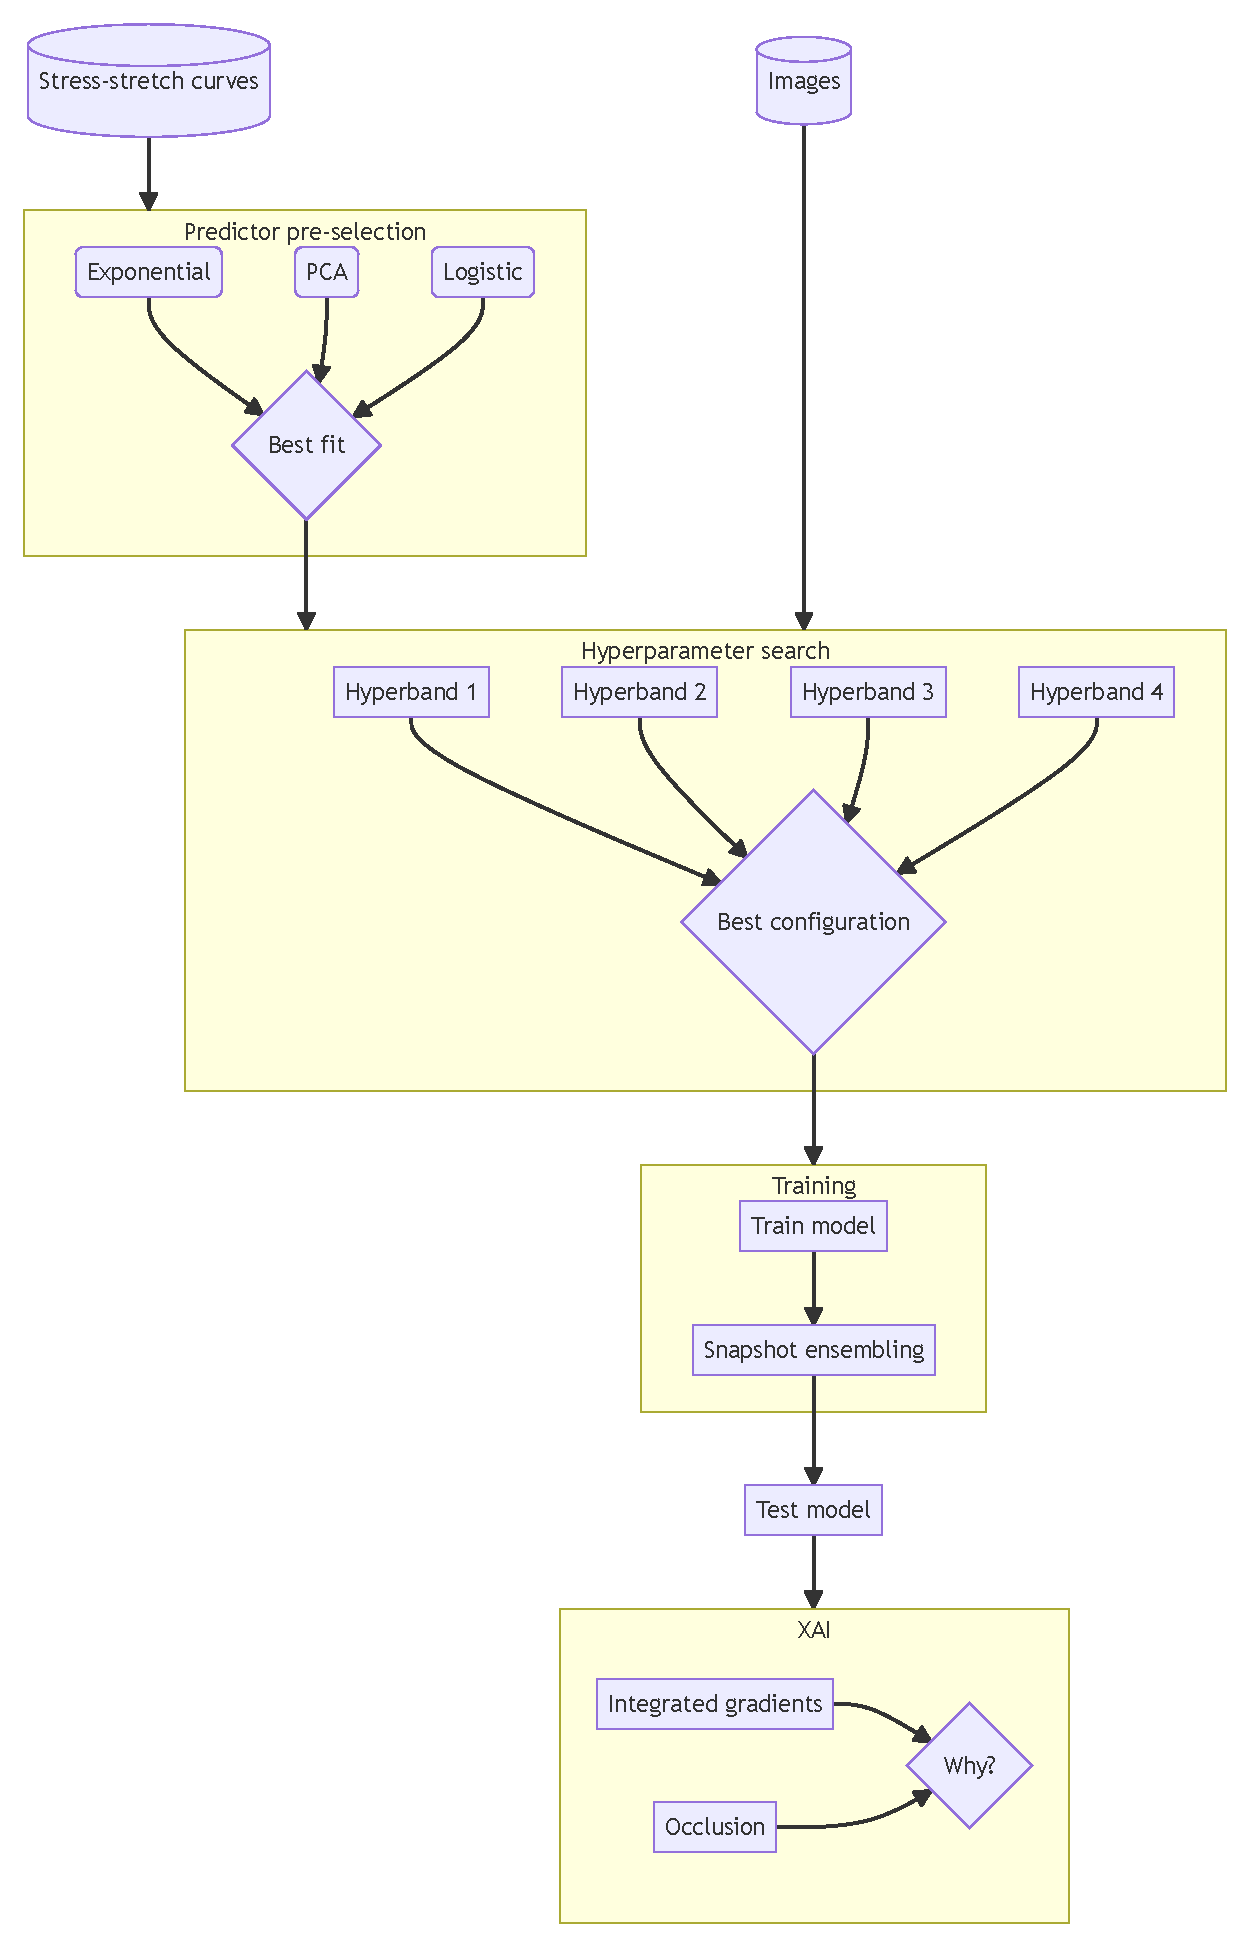
\includegraphics[height=\dimexpr\textheight-55.89pt\relax]{mermaid/skin_analysis.pdf}
    \caption[Flowchart of statistical analysis methods for \textsc{Skinstression}]{
        Flowchart of statistical analysis methods for \textsc{Skinstression}.
        Exponentials, principal component analysis (PCA) reconstructions, and logistic curves were fit to the stress-strain curves.
        The best-fitted model was used to create training targets.
        The targets and images were used as input for further training.
        The hyperparameter search was performed by four Hyperband studies and the best configuration was used for further training.
        After training, Snapshot Ensembling was used to build a final model.
        The final model is tested and interrogated using the XAI techniques integrated gradients and occlusion.
    }
    \label{fig:skin_stat_methods}
\end{figure*}

\subsection{Predictor pre-selection}
As discussed in \cref{sec:skin_predictors}, there are three predictor candidates.
These candidates are tested against the original strain-stress curves.

\subsubsection{Exponential and logistic curve}
The exponential and logistic models are fitted to all raw strain-stress curves.
The goodness of fit is determined by the coefficient of determination (\cref{subsec:coef_det}) and by eye.
A fit is considered good if it passes reasonably through all data points.
In particular, the exponential regime of the fit should describe the leg part of the curve.

\subsubsection{Principal component analysis}
PCA requires information on at least one axis to align between every curve.
The first step to achieve this is excluding all stretch values above the stretch of the maximum of the shortest curve.
\textcite{Soylu2022} did linear interpolation on the curves and restricted both stretch and stress to minim peak value.
PCA on two variables requires only one shared set of points.
Moreover, results of \citeauthor{Soylu2022} show knicks in the PCA reconstructions near the end of the curves, which could originate from a limited amount of datapoints or linear interpolation.
Therefore, in this study, a non-uniform, univariate, interpolating spline was fitted to all points and the stress was calculated from the spline at the stetch values of the curve with the lowest maximum stretch.
After PCA on the complete dataset, the explained variance per component was calculated and used as a method to find an appropriate number of principal components.
From these principal components, the curves where reconstructed using \cref{eq:pca}.
The goodness of fit is determined by the coefficient of determination (\cref{subsec:coef_det}) and by eye.
A fit is considered good if it passes reasonably through all data points and has few inflection points.

Only if PCA on the full dataset works reasonably well, it is possible to use PCA on a subset and use it to reconstruct another subset.
This would be useful if PCA was used to construct predictors, as using PCA results of the full dataset introduce information leakage from the test sets to the training set, because the components describe data from both subsets.
This is unlike Ref.~\cite{Soylu2022} where information leakage was not considered.\marginnote{Where to put PCA bias study?}

\subsection{Convolutional neural network}
The basis of the model originates from Liang \emph{et al.} \cite{Liang2017} and is adapted by Soylu \cite{Soylu2022}.
The model, a convolutional neural network, consists of five blocks.
The first block consists of a convolutional layer with a $\qty{3}{px}\times\qty{3}{px}$ kernel, taking in one channel and have 64 channels as output.
The output is then normalized per batch using BN (\cref{sec:bn}).
The normalized batch is passed through a ReLU (\cref{subsec:relu}) layer.
After activation, three $\qty{2}{px}\times\qty{2}{px}$ maxpool (\cref{subsec:maxpool}) layers are applied.
The next second block is like the first block, but with a $\qty{5}{px}\times\qty{5}{px}$ convolution kernel en just one maxpool layer.
The third block is like the second block, but with a $\qty{3}{px}\times\qty{3}{px}$ convolution kernel.
The fourth block is like the second and third block, but with a $\qty{6}{px}\times\qty{6}{px}$ and without a maxpool layer.

The fifth block flattens the input and consists of a two linear layers.
The first linear layer maps 64 nodes to $N_\mathrm{nodes}$ nodes.
After the first linear layer, BN and ReLU activation is applied.
The second linear layer maps $N_\mathrm{nodes}$ nodes to 3 nodes.
A linear activation function ensures the output is continuous and unaltered.
The model is shown in \cref{fig:model}

\begin{figure*}
    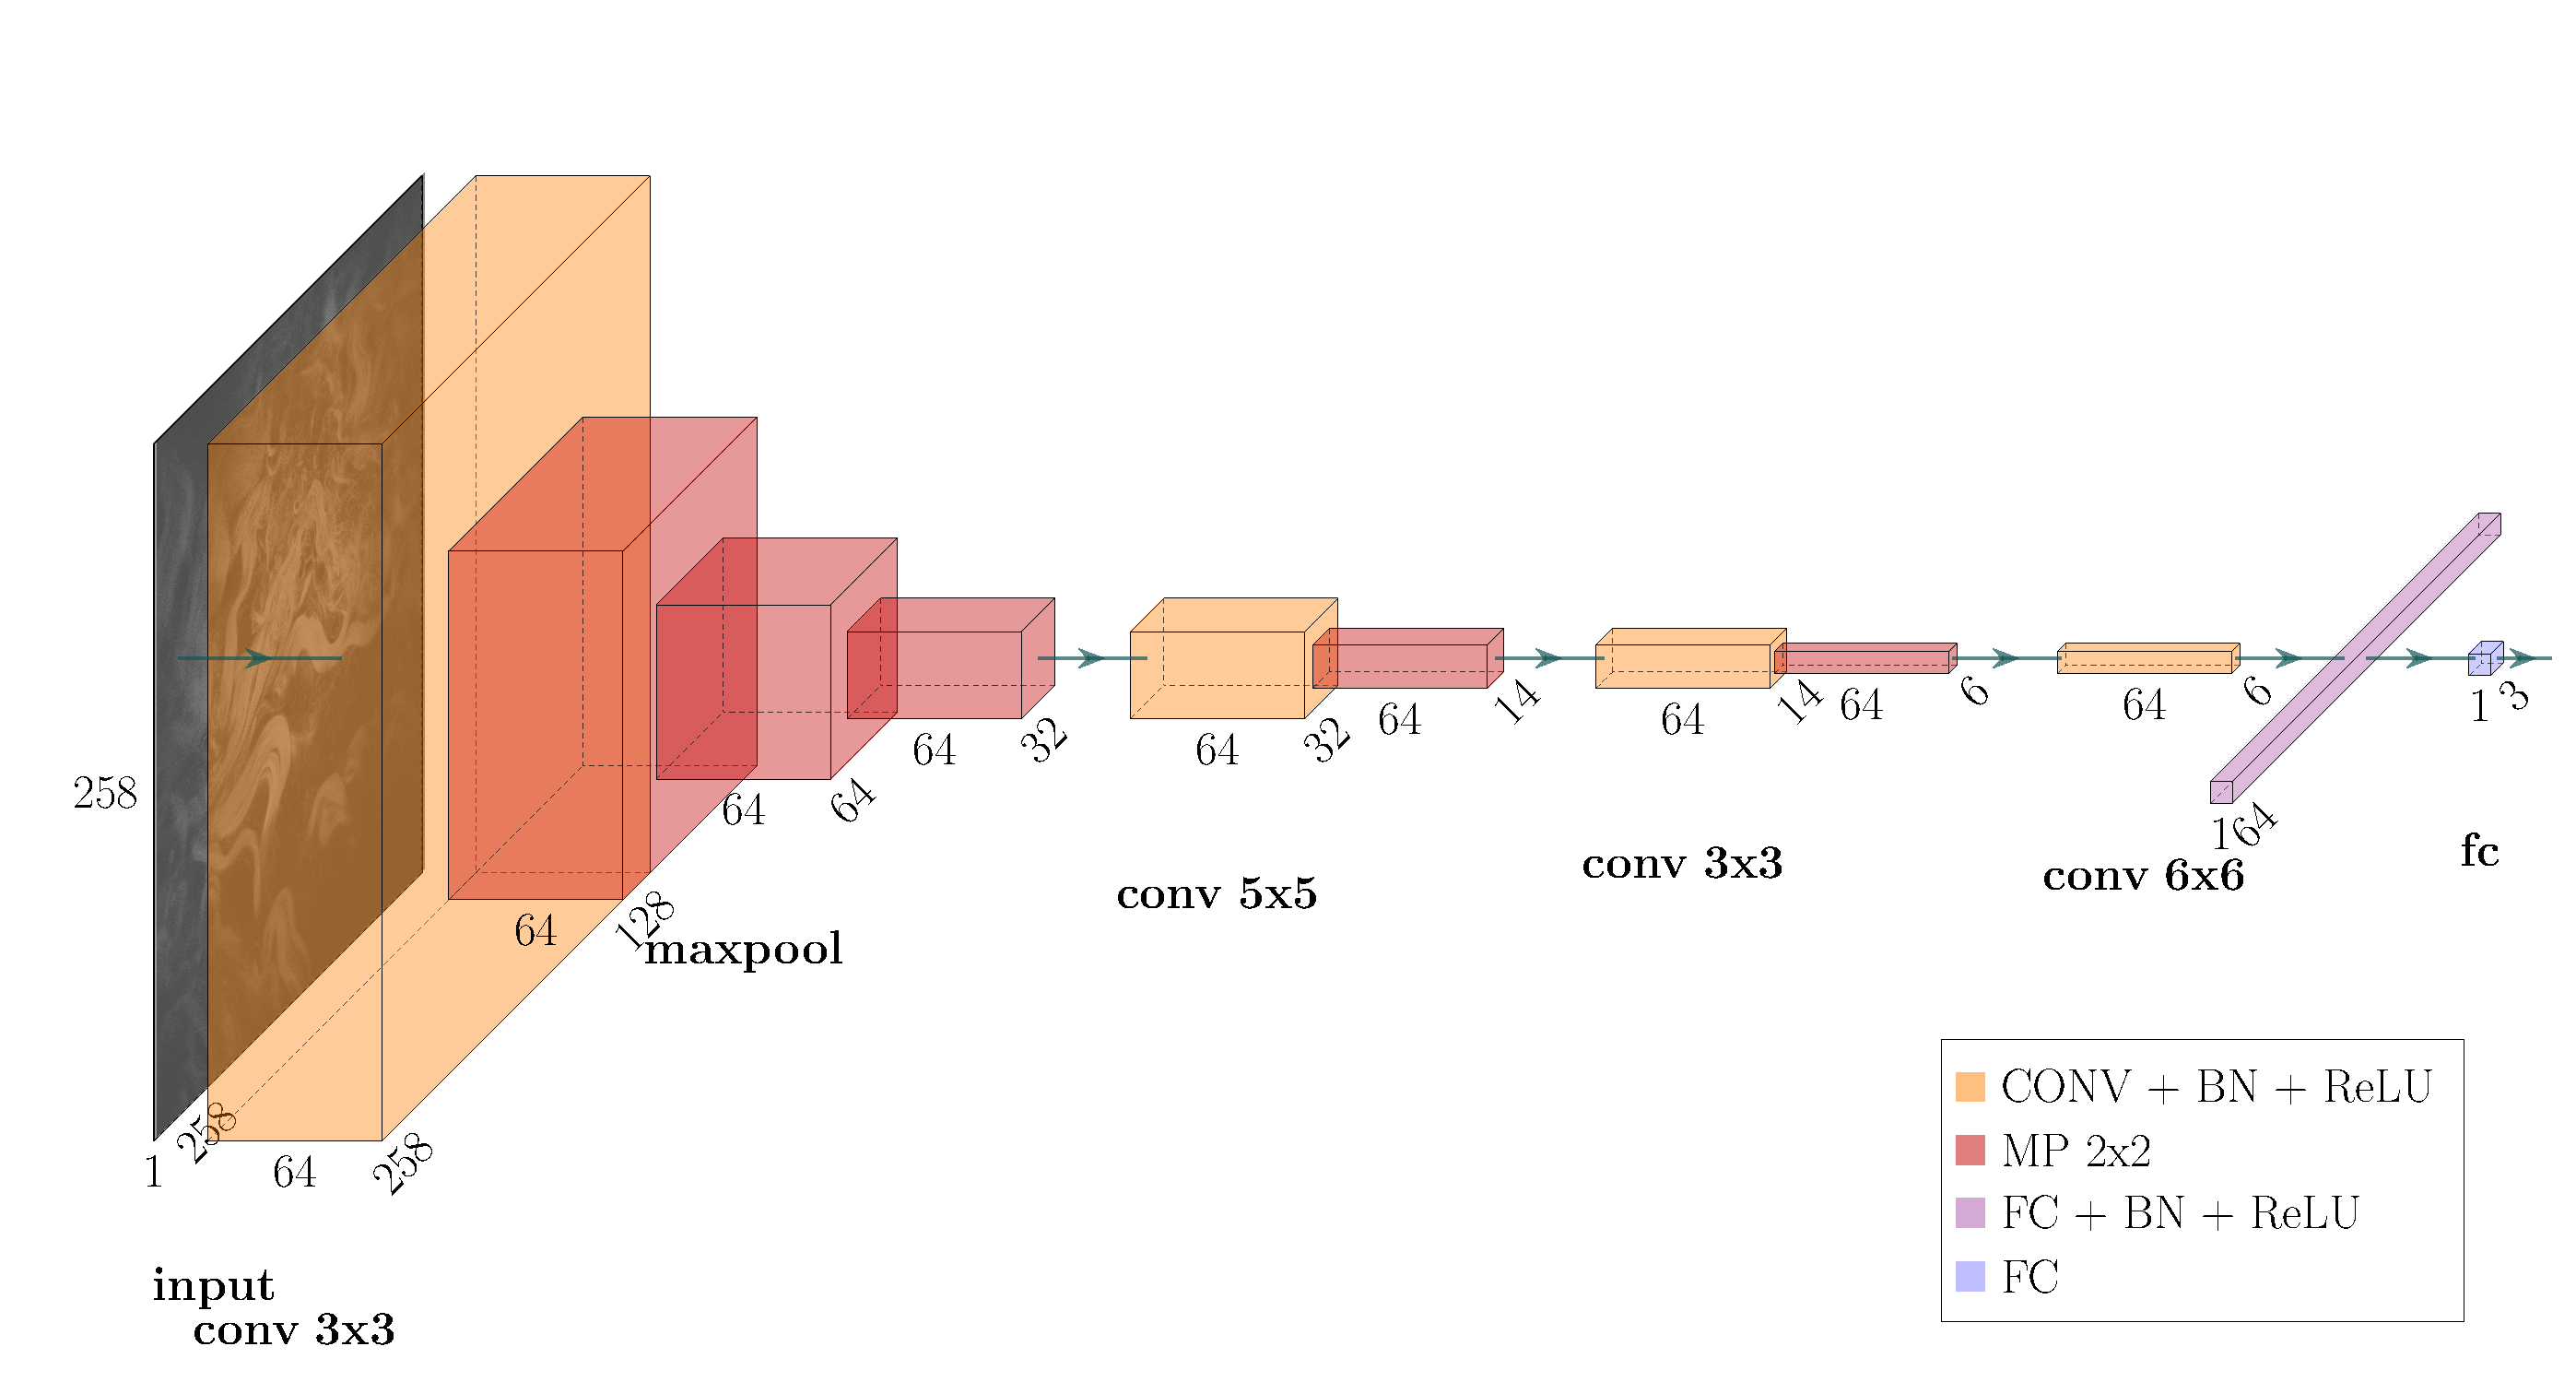
\includegraphics{skinstression/images/skinstression.pdf}
    % \input{PlotNeuralNet/examples/Skinstression/skinstression-new.tex}
    \caption[Network architecture]{
        The convolutional neural network consists of five blocks.
        The first four blocks contain convolution, maxpooling, and batch normalization layers.
        The last block contains a fully connected network.
        It requires an input of $\qty{258}{px}\times\qty{258}{px}$ to get a vector of length 3 as output.
    }
    \label{fig:model}
\end{figure*}

The dropout layers in \cite{Soylu2022} are replaced by BN layers.
Bias of all layers preceding BN layers have been set to zero.

The neural network weights are initialized according to the method described by \textcite{He2015a}, using a uniform transform.

\subsection{Hyperparameter optimization}
To find the optimal set of hyperparameters, the Hyperband algorithm with 300 trials was used.
To allow trials to warmup, a minimum of 100 epochs were allowed.
To limit the trial duration, a maximum of 3000 epochs were allowed.
The number of trials were reduced with a reduction factor of $\eta=4$.
Trial parameters were sampled using the multivariate TPE algorithm.
See \cref{subsec:conf_skin} for a summary of configuration search space $\mathcal{C}$.
Every trial used the complete dataset after data preparation (\cref{sec:skin_data_prep}).

Four different Hyperband searches were performed, see \cref{tab:skin_studies}.
Search 1 will serve as a benchmark study.
It contains a few data augmentations that are assumed to not alter the physical context of the image.
That is, force is exerted on the tissue in the horizontal direction in the image.
Therefore, flipping the image either vertically or horizontally is assumed to not change the stretch behaviour.
Both flipping operations occur with a probability of $0.5$.
Moreover, the images' intensity is randomly changed between x\% and x\%.\marginpar{By what fraction is the intensity changed?}
Search 2 includes CLAHE to enhance the image.
Moreover, random $700\times700$ cropping is added to further artificially increase the number of available images to train on.
Also included is the ability to weight the loss per target variable, to penalize hard variables more than easy variables.
Search 3 includes the Yeo-Johnson transformation to see how input normalization affects the training outcome.
Search 4 adds random sharpness and gaussian blurring to increase the training set variability.
It also includes random rotation from \ang{0} to \ang{90}.
The random rotation along with flipping in two directions ensures all possible rotations.
The Yeo-Johnson transform from search 3 was excluded in search 4.

\begin{table}
    \caption[\textsc{Skinstression} hyperparameter search studies]{
        The hyperparameter searches performed.
        Hyperparameters are grouped by operation type (image preprocessing, image augmenting, target weighting) and in applied order.
        Every study, more is added, except for search 4 where the Yeo-Johnson transform was removed.
        Note this table does not describe the full search space.
        Every search is done with the search space described in \cref{tab:conf_skin}.
    }
    \label{tab:skin_studies}
    \begin{tabular}{rcccc}
        \toprule
        Search                         & 1      & 2      & 3      & 4      \\
        \midrule
        CLAHE                          & \xmark & \cmark & \cmark & \cmark \\
        Yeo-Johnson transform          & \xmark & \xmark & \cmark & \xmark \\
        \midrule
        Random $700\times700$ cropping & \xmark & \cmark & \cmark & \cmark \\
        Intensity jitter               & \cmark & \cmark & \cmark & \cmark \\
        Random horizontal flip         & \cmark & \cmark & \cmark & \cmark \\
        Random vertical flip           & \cmark & \cmark & \cmark & \cmark \\
        Random sharpness               & \xmark & \xmark & \xmark & \cmark \\
        Random gaussian blur           & \xmark & \xmark & \xmark & \cmark \\
        Random rotation                & \xmark & \xmark & \xmark & \cmark \\
        \midrule
        Target variable weighting      & \xmark & \cmark & \cmark & \cmark \\
        \bottomrule
    \end{tabular}
\end{table}

\subsection{Training}
Using the best configuration for hyperparameter optimization, a model is trained further for a total of $N$\marginnote{How many exactly?} epochs.
The learning rate scheduler was cosine annealing with warm restarts to allow for model ensembling later during inference (\cref{subsec:model_ensembling}).

\subsection{Model selection}
MISSCHIEN MODEL ENSEMBLING EN VALIDATION SET GEBRUIKEN VOOR VINDEN VAN BESTE AANTAL MODELS?
The last $N$\marginnote{How many again?} models are ensembled together

\section{Supplementary materials}
\subsection{Code}
The implementation of \textsc{Skinstression} can be found at \href{https://github.io/siemdejong/shg-strain-stress}{\faIcon{github} siemdejong/shg-strain-stress}.
The context and container diagram are depicted in \cref{app:skin_c4}.
\chapter{Results}

\section{Participants}

Earlier studies (refs) include 18 individuals (5 men, 4 women, and 6 unknown).
Abdomen data was excluded, because the strain-stress curves differ significantly from the thigh.
All thigh data is included, which is different from the original study, where only the 48 latest samples were used.
These considerations result in data including 15 individuals (5 men, 4 women, 3 unknown).
Ages range from 61 to 94.
Skin tissue is cut from the thigh and cut in multiple pieces of roughly the same shape.\marginpar{protocol?}
From every skin tissue piece, strain-stress curves are measured.
The number of measured strain-stress curves range from 1 to 13.
The source of data is summarized in table~\ref{tab:source_of_data}
\begin{table}
    \centering
    \caption[Source of data]{
        The selected individuals and their sex, age and number of strain-stress curves.
        - denotes unknown data.
    }
    \label{tab:source_of_data}
    \begin{tabular}{lllr}
        \toprule
        person & sex    & age & \# curves \\
        \midrule
        4      & -      & -   & 1         \\
        5      & male   & 61  & 1         \\
        6      & male   & 66  & 2         \\
        7      & male   & 79  & 1         \\
        8      & male   & 77  & 1         \\
        9      & male   & 75  & 1         \\
        10     & female & 94  & 1         \\
        11     & -      & -   & 1         \\
        12     & -      & -   & 1         \\
        13     & male   & 82  & 3         \\
        14     & female & 90  & 4         \\
        15     & female & 87  & 5         \\
        16     & male   & 95  & 12        \\
        17     & male   & 83  & 13        \\
        18     & female & 88  & 9         \\
        \bottomrule
    \end{tabular}
\end{table}
\chapter{Discussion}

TODO?:
\begin{enumerate}
    \item collagen is viscoelastic and is therefore timedependent.
    \item discard strain-stress curve outliers (using PCA?)
    \item (random cropping has a higher probability of including pixels in the middle region)
    \item WHY DEEP LEARNING?
    \item train/val/test diff of 'source of data' fig
\end{enumerate}

\section{Logistic curve fits stress-strain curves better than an exponential or PCA}
With an $\overline{R^2} \approx \num{0.9979 \pm 0.0039}$, the logistic curve fits stress-strain data (\cref{fig:logistic_fits}) better than the exponential or PCA ($\overline{R^2} \approx \num{0.9927 \pm 0.0022}$, \cref{fig:pca_fits}).
The exponential does not fit the plateau that is often present at the end of a stress-strain curve (\cref{fig:exp_fits}).
This plateau is essential to the skin tissue dynamics.
It shows at which point the integrity of the collagen matrix breaks down, \ie when the skin cannot resist the force acting on it.
PCA had to be done after truncating all curves to maximum strain of the curve with the smallest maximum strain.
This resulted in PCA fits that only described the first region of the curve.
Moreover, to fairly create PCA fits, PCA has to be trained on a training set and values extracted from the test set must be projected onto this test set.
This may lead to generalizability problems.
For these reasons, the logistic curve parameters are used as a predictors.

\section{Shannon entropy is a better measure to exclude noise than kurtosis}\label{sec:disc_ent_vs_kur}
Measures to be used to exclude noise are kurtosis (\cref{fig:skin_kurtosis_depth}) and Shannon entropy (\cref{fig:skin_entropy_depth}).
For rather homogeneous images like stack 8, kurtosis is able to characterize the fogginess, while entropy finds images of equal quality.
However, for well-structured tissue like stack 11, 12, 13 and 4, entropy recognizes faint images and qualifies them as bad.
This is particularly useful for images that did not include any useful information (like stack 37).
Kurtosis does not succeed to distinguish dark images from bright ones.
Kurtosis also has the tendency to fluctuate, which is unexpected between subsequent slices.
For these reasons, Shannon entropy has been used to choose the top $N_\mathrm{best}$ images.

\section{Stretch information can be extracted from SHG microscopy images}
\Cref{fig:skinstression-train-logistic-curves} shows that for most images, it is possible to extract stretch information.
Using the model, ten images from different stacks of the train set yield a stress-strain curve with $R^2>0.9$.
This shows that stretch information is present, even in the drastically downsized images.

\section{The model does not generalize well}
Although the train results were promising, the test results of \cref{fig:skinstression-test} show a lack of generalizability.
Only two images from different stacks of the test set yield a stress-strain curve with $R^2=0.99$.
This shows that the training set does not include enough features similar to the features in the test set.
More images need to be included in the training set for the model to generalize well to held-out test cases.

\section{Artificially increasing collagen density increases maximum stress prediction and stiffness and vice versa}
As shown in \cref{fig:pred_output_attack}, artificially filling holes with collagen increases the maximum stress significantly and increases the maximum Young's modulus slightly.
This is expected, as an increase in collagen density generally is an increase in the number of springs in the system.
Adding springs increases the stiffness.
The increase in maximum stress is likely due to the addition of springs supporting each other dividing the load.
On the contrary, with comparable reasoning, artificially decreasing the collagen density by duplicating a hole lowers both the maximum stress and Young's modulus.

\section{Future studies}
\subsection{Perform cross validation and increase data variance}
In this study, no cross validation is performed.
Training a network on different training subsets might increase the performance on the test set.
The test set might include patterns that were not present in the training set and therefore will not activate critical parts of the neural network.
The split between training and test sets should be made such that the training set has high variance and is thus a reasonably good estimate of the whole population, without knowing test set images.

Therefore, the training set should also include images from human skin that is damaged in any way.
For example, damaged tissue is caused by smoking \cite{Lipa2021} or wounds that left behind scars with an increased tensile strength \cite{Wilkinson2020}.
Moreover, aging drastically impacts skin tissue integrity.
It is unknown if stretch of young skin tissue is predicted well by the neural network.
Therefore, the neural network should only be used to predict from old skin tissue.

Skin tissue from other body parts might show different stretch properties.
Therefore, it is unknown if the stretch of skin tissues other than from the upper leg can be predicted.

Lastly, to increase variance, more images of skin tissue from more individuals should be included.

\subsection{Split dataset before image and target transformations}
LDS should only be performed on the training set, independently from the validation and test set.
This is to prevent leaking data to the training set.
By design, the software constructs train, validation and test split datasets with data transformations, including target transformations such as LDS and the Yeo-Johnson transformation.
Every split in fact contains all $N_\mathrm{best}$ images and includes transformations.
Just before constructing a dataloader, the datasets are split by index, leaving the dataloaders with non-overlapping data.
In future studies, the dataset should be split into subsets with their specific transformations applied.
While this increases training fairness, it is expected to decrease performance, as information from the test set is not leaked to the training set.

Moreover, the split indices were generated by shuffling $\{1,\, 2,\, 3,\, \ldots,\, N_\mathrm{images}\}$ and splitting the indices at \qty{80}{\percent}, giving indices for the training/validation and test set.
Next, a new set of indices, $\{1,\, 2,\, 3,\, \ldots,\, \qty{80}{\percent} \cdot N_\mathrm{images}\}$ is shuffled and split at \qty{80}{\percent}, yielding indices for the training and validation set.
All splits were stratified by person, meaning the shuffle was done in such a way that images from the same person could not live in the training or validation set.
This way, the training and validation set had overlap with the test set, but not with each other.
To create an independent test set, the operation
\begin{equation}\label{eq:skin_newtest_idx}
    \texttt{actual test} = \texttt{test} - (\texttt{train} \cup \texttt{validation})
\end{equation}
was performed.
However, this does not make use of the full dataset.
To achieve that, \cref{eq:skin_newtest_idx} should be rewritten as
\begin{equation}
    \texttt{actual test} = \{1,\, 2,\, 3,\, \ldots,\, N_\mathrm{images}\} - (\texttt{train} \cup \texttt{validation}).
\end{equation}
This version of \texttt{actual test} has one major drawback, which is that the \qty{20}{\percent} highest indices are reserved for the test set, effectively excluding them from the shuffle.
A future study should perform a train/validation split on shuffled indices after splitting off the test set.

\subsection{Excluding noise and denoising on stack level}
Currently, the stacks are truncated by taking the top $N_\mathrm{best}$ images of a stack which effectively excludes noisy slices.
However, if a full z-stack is noisy, noisy images are still included.
These noisy images may still harm training and could be excluded, too.
Possibly, excluding noisy stacks can for example be done by calculating the Shannon entropy of all truncated stacks and include stacks with the highest entropy.

In addition to noise exclusion, denoising stacks with three-dimensional N2V or individual slices with N2V2\footnote{At the time of writing, N2V2 is not yet compatible with three-dimensional images.} could increase model performance.
This is because noise can occlude patterns that describe stretch information.

\subsection{Using three-dimensional images}
The current model relies on single images belonging to stacks.
All structural information in the depth direction is disregarded by the neural network.
If the neural network is redesigned to recognize patterns in three dimensions, it is expected to better predict the skin stretch properties.

\subsection{Using full-size images}
The microscope outputting the SHG images has a much larger resolution.\marginnote{How much larger?}
The method in this study did not make use of this resolution.
Higher resolution images contain more information on the collagen structure, and are therefore expected to increase the performance.
The presented model has to be redesigned to accept images larger than $258\times258$.
Moreover, raw data is stored with a larger dynamic range (16-bit instead of 8-bit).
Being able to see small differences in neighbouring pixel intensities increases the available information \eg in darker regions, where collagen is sparse, but still significantly present.

\subsection{Weighting samples by goodness of target fit}
The neural network learns from targets that are a result of logistic curves fitted to a series of datapoints.
The goodness of fit differs between curves.
Fits that do not describe the data well should not negatively impact the model training.
One way to achieve this is by reweighting the loss function as
\begin{equation}
    \mathcal{L}_{R^2\,\mathrm{weighted}} =
    \begin{cases}
        \mathcal{L} / \left(R^2\right)^b & \text{if } R^2 > a     \\
        \mathcal{L} / a^b                & \text{if } R^2 \leq a,
    \end{cases}
\end{equation}
where $a$ is a lower bound to $R^2$ and $b > 0$ can influence the amount of weighting.


% \defbibnote{bibnote}{Here are the references in citation order.\par\bigskip} % Prepend this text to the bibliography
% \printbibliography[heading=bibintoc, title=Bibliography, prenote=bibnote] % Add the bibliography heading to the ToC, set the title of the bibliography and output the bibliography note
\printbibliography[heading=bibintoc, title=References] % Add the bibliography heading to the ToC, set the title of the bibliography and output the bibliography note


\pagelayout{wide} % No margins
\addpart{Title of the Part}
\pagelayout{margin} % Restore margins

\chapter{Second Chapter}

\blindtext

\appendix % From here onwards, chapters are numbered with letters, as is the appendix convention

\pagelayout{wide} % No margins
\addpart{Appendix}
\pagelayout{margin} % Restore margins

\chapter{Some more blindtext}

\blindtext

%----------------------------------------------------------------------------------------

\backmatter % Denotes the end of the main document content
\setchapterstyle{plain} % Output plain chapters from this point onwards

%----------------------------------------------------------------------------------------
%	BIBLIOGRAPHY
%----------------------------------------------------------------------------------------

% The bibliography needs to be compiled with biber using your LaTeX editor, or on the command line with 'biber main' from the template directory

% \defbibnote{bibnote}{Here are the references in citation order.\par\bigskip} % Prepend this text to the bibliography
% \printbibliography[heading=bibintoc, title=Bibliography, prenote=bibnote] % Add the bibliography heading to the ToC, set the title of the bibliography and output the bibliography note

%----------------------------------------------------------------------------------------
%	INDEX
%----------------------------------------------------------------------------------------

% The index needs to be compiled on the command line with 'makeindex main' from the template directory

\printindex % Output the index

\end{document}
